Para poder enfrentarnos con garantías al desarrollo del proyecto es
necesario conocer una serie de conceptos relacionados con el sonido y
la música en general, y conceptos sobre análisis de señales que
explicaremos a lo largo de este capítulo.

\section{El sonido}
Un \textbf{sonido} es una vibración que se propaga por un medio
elástico en forma de onda. Estas vibraciones se transmiten de forma
longitudinal, esto es, en la misma dirección en la que se propaga la
onda. El medio más común para la transmisión del sonido es el
\textbf{aire}. 

El sonido, en su forma más simple, se compone de una sola onda
sinusoidal básica, con las características tradicionales: amplitud,
frecuencia y fase. Una \textbf{onda sinusoidal} es aquella cuyos
valores se calculan utilizando funciones seno.

\subsection{Frecuencia y tono}
La \textbf{frecuencia} mide el número de oscilaciones de la onda por
unidad de tiempo. Por regla general, se utiliza el \textbf{hercio}
como unidad de medida de frecuencia, que indica la cantidad de
repeticiones por segundo. La frecuencia determinará la \textbf{altura}
del sonido, es decir, cómo de grave o agudo es. Los sonidos graves
tienen una frecuencia baja, mientras que los sonidos agudos tienen una
frecuencia alta.

A lo largo de los años se ha establecido un estándar de referencia que
establece que la nota \textit{la} que se encuentra encima del
\textit{do} central del piano debe sonar a 440 hercios de
frecuencia. Esta medida se utiliza a la hora de afinar los
instrumentos, de modo que si al tocar la nota \textit{la} se detecta
un tono con una frecuencia de 440 hercios, entonces el instrumento
estará bien afinado.

El espectro audible por las personas lo conforman las
\textbf{audiofrecuencias}, esto es, el conjunto de frecuencias que
pueden ser percibidas por el oído humano. 

\begin{figure}[h]
  \centering
  
\includegraphics[scale=0.8]{conceptos/rango_freq}
  \caption{Rango de frecuencias de sonido}
\end{figure}


Un oído sano y joven es capaz de detectar sonidos a partir de los 20
hercios. Los sonidos por debajo de esa frecuencia se conocen como
\textbf{infrasonidos}. Por otro lado, el límite auditivo en
frecuencias altas varía mucho con la edad: un adolescente puede oir
sonidos con frecuencias hasta los 18kHz, mientras que un adulto de
edad media solo suele llegar a captar sonidos de hasta 13kHz. El
límite genérico superior se establece en 20kHz, por encima de los
cuales los sonidos se denominan \textbf{ultrasonidos}.


\subsection{Amplitud}
La \textbf{amplitud} representa la energía que transporta la
onda. Cuando un instrumento u otro objeto genera una vibración, la
amplitud es la cantidad de movimiento que esa vibración genera.
Podría equipararse (de forma no estricta) a la intensidad del sonido:
cuanto mayor sea la amplitud, más fuerte se oirá el sonido.

\subsection{Fase}
Por último, la \textbf{fase} ($\varphi$) indica el desplazamiento
horizontal de la onda respecto del origen. Si la fase de una onda no
es cero, entonces parecerá que está \textit{desplazada} hacia la
derecha, si la fase es positiva, y hacia la izquierda si la fase es
negativa.
\begin{figure}[h]\centering
    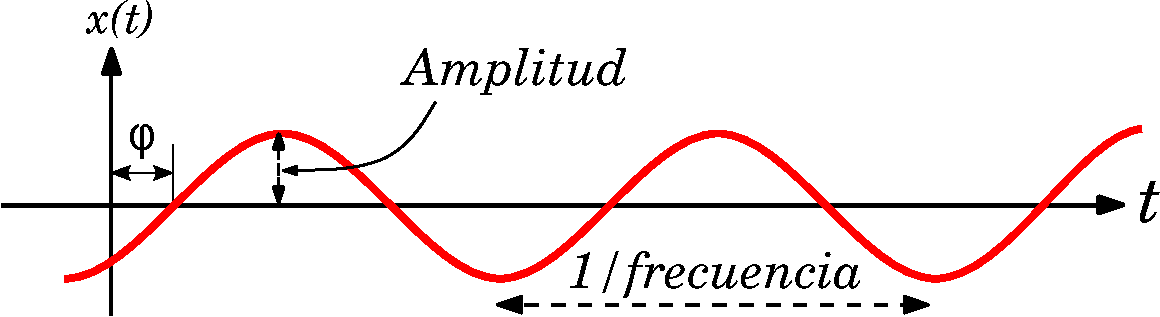
\includegraphics[scale=0.7]{conceptos/onda}
    \caption{Componentes de una señal senoidal básica}
\end{figure}
\section{Descomposición de sonidos}
Para desarrollar oFlute nos interesa conocer la altura de la nota que
está tocando la flauta en un instante concreto. Para un tono puro,
podríamos conocer la altura fijándonos en su frecuencia. El problema
es que, en la naturaleza, \textbf{no existen} los tonos puros, sino
que los sonidos se componen de multitud de tonos de diferentes
amplitudes, frecuencias y fases. 

Afortunadamente, la teoría dicta que cualquier tono complejo puede
descomponerse como suma de tonos puros de distintas amplitudes, fases
y frecuencias, llamados \textbf{parciales}. La menor de todas las
frecuencias de los parciales se conoce como \textbf{frecuencia
  fundamental}, y es la que que dicta la altura general del sonido --
\textit{general}, ya que aunque el resto de frecuencias puede
corresponder a otras notas, es la altura de la frecuencia fundamental
la que mayor relevancia tiene en el sonido.

Un subconjunto de esos parciales, conocidos como \textbf{armónicos},
tienen frecuencias múltiplos de la frecuencia fundamental. Estos
armónicos sirven para enriquecer el sonido y, sobre todo, determinar
el \textbf{timbre musical} del origen del sonido: dos instrumentos (o
personas) pueden estar tocando la misma nota y emitir la misma
frecuencia fundamental, pero será el conjunto total de armónicos el
que nos ayude a distinguir qué instrumento está emitiendo el sonido.

Así pues, el objetivo es encontrar una forma de descomponer una señal
(el sonido) en sus componentes y analizar sus frecuencias, buscando la
frecuencia fundamental, que nos informará de la nota que se está tocando. 

\subsection{Representación gráfica de sonidos}

Las representación habitual de las señales se hace en el
\textbf{dominio del tiempo}, es decir, podemos observar cómo la señal
cambia a lo largo del tiempo, viendo el valor de su \textbf{amplitud}
en cada instante. Por otro lado, la representación en el
\textbf{dominio de la frecuencia} nos permite analizar una señal
respecto a las frecuencias que la componen, dividiendo la señal en sus
componentes.

En la figura \ref{fig:wavespectral} podemos comparar la representación de
un sonido en el dominio del tiempo, en \textbf{forma de ondas}, tal y
como aparecería en un osciloscopio, frente a su representación en
\textbf{forma espectral}, en la que el eje vertical indica la
frecuencia, y la intensidad del color indica la intensidad de esa
componente frecuencial en el sonido.

\begin{figure}[h!]
  \centering
  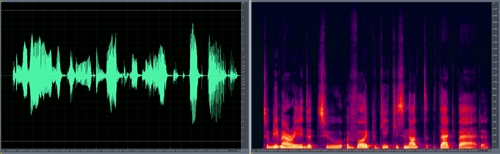
\includegraphics[scale=0.8]{conceptos/wave_spectral}
  \caption{Forma de ondas vs representación espectral}
  \label{fig:wavespectral}
\end{figure}

\subsection{Herramientas de descomposición de señales}

La herramienta fundamental a la hora de descomponer una señal
periódica como puede ser un sonido en sus parciales o armónicos es el
\textbf{análisis armónico} o \textbf{análisis de Fourier}. Esta rama
del análisis matemático estudia la representación de funciones o
señales como superposición de ondas básicas, y hoy en día se aplica en
innumerables campos de la ciencia, desde el procesamiento de señales,
como es nuestro caso, a la neurociencia. 

Una de las herramientas más conocidas de este área es la
\textbf{transformada de Fourier}, que nos permite pasar una señal del
dominio del tiempo al de la frecuencia. La transformada de Fourier es
una aplicación matemática
